
\documentclass[hyperref={pdfpagelabels=false}, compress]{beamer}
%\let\Tiny=\tiny

\usepackage[T1]{fontenc} 
\usepackage{lmodern}
\usepackage{graphicx}
\usepackage{hyperref}
\usepackage{url}
%\usepackage[style=footnote-dw]{biblatex}
%\usepackage[style=apa]{biblatex}
\usepackage{BeamerColor}

%\usepackage{natbib}
%\bibliographystyle{apalike}

%\mode<presentation>
%{  
	\usetheme{Frankfurt}
  	\usecolortheme[named=firebrick4]{structure}
	%\usecolortheme{beaver}
	%\usecolortheme{lily}
  	\useinnertheme{circles}
  	\usefonttheme[onlymath]{serif}
  	\setbeamercovered{transparent}
  	\setbeamertemplate{blocks}[rounded][shadow=true]
	\setbeamertemplate{footline}[page number]{}
	\setbeamertemplate{navigation symbols}{}
	%\setbeamerfont{footnote}{size=\tiny}
%}

%\bibliography{References} 

\newenvironment{changemargin}[2]{%
  \begin{list}{}{%
    \setlength{\topsep}{0pt}%
    \setlength{\leftmargin}{#1}%
    \setlength{\rightmargin}{#2}%
    \setlength{\listparindent}{\parindent}%
    \setlength{\itemindent}{\parindent}%
    \setlength{\parsep}{\parskip}%
  }%
  \item[]}{\end{list}}

\renewcommand{\familydefault}{\sfdefault}

%%%%%%%%%%

\title{dictyBase @ Northwestern University}
\author{\textit{Dictyostelium discoideum}}

%\date[December 25, 1001]
\date

\begin{document}

\frame{\titlepage}

\section[Overview]{}
\frame{\tableofcontents}

%%%%%%%%%%

\section{Blocks}
\begin{frame}
	\frametitle{}
	
	\begin{block}{}
		\begin{itemize}
			\item Blocks example
		\end{itemize}
	\end{block}
\end{frame}

%%

\section{Slide animation and Footer}
\begin{frame}
	\frametitle{}
	
	\begin{itemize}
		\item<1> Hello World !
	\end{itemize}
	
\let\thefootnote\relax\footnotetext{Acknowledgment: NCBI}
\end{frame}

%%

\section{Graphics}
\begin{frame}
	\begin{center}
		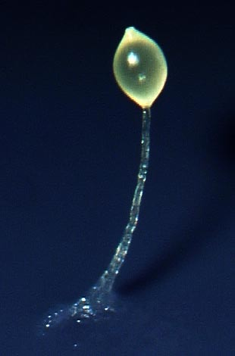
\includegraphics[scale=0.45]{dicty_stalk.png}
	\end{center}
\end{frame}

%%%%%%%%%%

\end{document}
